\documentclass[a4paper, 14pt]{extarticle}
\usepackage{float}
% Поля
%--------------------------------------
\usepackage{geometry}
\geometry{a4paper,tmargin=2cm,bmargin=2cm,lmargin=3cm,rmargin=1cm}
%--------------------------------------


%Russian-specific packages
%--------------------------------------
\usepackage[T2A]{fontenc}
\usepackage[utf8]{inputenc} 
\usepackage[english, main=russian]{babel}
%--------------------------------------

\usepackage{textcomp}

% Красная строка
%--------------------------------------
\usepackage{indentfirst}               
%--------------------------------------             


%Graphics
%--------------------------------------
\usepackage{graphicx}
\graphicspath{ {./images/} }
\usepackage{wrapfig}
%--------------------------------------

% Полуторный интервал
%--------------------------------------
\linespread{1.3}                    
%--------------------------------------

%Выравнивание и переносы
%--------------------------------------
% Избавляемся от переполнений
\sloppy
% Запрещаем разрыв страницы после первой строки абзаца
\clubpenalty=10000
% Запрещаем разрыв страницы после последней строки абзаца
\widowpenalty=10000
%--------------------------------------

%Списки
\usepackage{enumitem}

%Подписи
\usepackage{caption} 

%Гиперссылки
\usepackage{hyperref}

\hypersetup {
	unicode=true
}

%Рисунки
%--------------------------------------
\DeclareCaptionLabelSeparator*{emdash}{~--- }
\captionsetup[figure]{labelsep=emdash,font=onehalfspacing,position=bottom}
%--------------------------------------

\usepackage{tempora}

%Листинги
%--------------------------------------
\usepackage{listings}
\lstset{
  basicstyle=\ttfamily\footnotesize, 
  %basicstyle=\footnotesize\AnkaCoder,        % the size of the fonts that are used for the code
  breakatwhitespace=false,        % sets if automatic breaks shoulbd only happen at whitespace
  breaklines=true,                 % sets automatic line breaking
  captionpos=t,                    % sets the caption-position to bottom
  inputencoding=utf8,
  frame=single,                    % adds a frame around the code
  keepspaces=true,                 % keeps spaces in text, useful for keeping indentation of code (possibly needs columns=flexible)
  keywordstyle=\bf,       % keyword style
  numbers=left,                    % where to put the line-numbers; possible values are (none, left, right)
  numbersep=5pt,                   % how far the line-numbers are from the code
  xleftmargin=25pt,
  xrightmargin=25pt,
  showspaces=false,                % show spaces everywhere adding particular underscores; it overrides 'showstringspaces'
  showstringspaces=false,          % underline spaces within strings only
  showtabs=false,                  % show tabs within strings adding particular underscores
  stepnumber=1,                    % the step between two line-numbers. If it's 1, each line will be numbered
  tabsize=2,                       % sets default tabsize to 8 spaces
  title=\lstname                   % show the filename of files included with \lstinputlisting; also try caption instead of title
}
%--------------------------------------

%%% Математические пакеты %%%
%--------------------------------------
\usepackage{amsthm,amsfonts,amsmath,amssymb,amscd}  % Математические дополнения от AMS
\usepackage{mathtools}                              % Добавляет окружение multlined
\usepackage[perpage]{footmisc}
%--------------------------------------

%--------------------------------------
%			НАЧАЛО ДОКУМЕНТА
%--------------------------------------

\begin{document}

%--------------------------------------
%			ТИТУЛЬНЫЙ ЛИСТ
%--------------------------------------
\begin{titlepage}
\thispagestyle{empty}
\newpage


%Шапка титульного листа
%--------------------------------------
\vspace*{-60pt}
\hspace{-65pt}
\begin{minipage}{0.3\textwidth}
\hspace*{-20pt}\centering

\includegraphics[width=\textwidth]{emblem}
\end{minipage}
\begin{minipage}{0.67\textwidth}\small \textbf{
\vspace*{-0.7ex}
\hspace*{-6pt}\centerline{Министерство науки и высшего образования Российской Федерации}
\vspace*{-0.7ex}
\centerline{Федеральное государственное бюджетное образовательное учреждение }
\vspace*{-0.7ex}
\centerline{высшего образования}
\vspace*{-0.7ex}
\centerline{<<Московский государственный технический университет}
\vspace*{-0.7ex}
\centerline{имени Н.Э. Баумана}
\vspace*{-0.7ex}
\centerline{(национальный исследовательский университет)>>}
\vspace*{-0.7ex}
\centerline{(МГТУ им. Н.Э. Баумана)}}
\end{minipage}
%--------------------------------------

%Полосы
%--------------------------------------
\vspace{-25pt}
\hspace{-35pt}\rule{\textwidth}{2.3pt}

\vspace*{-20.3pt}
\hspace{-35pt}\rule{\textwidth}{0.4pt}
%--------------------------------------

\vspace{1.5ex}
\hspace{-35pt} \noindent \small ФАКУЛЬТЕТ\hspace{80pt} <<Информатика и системы управления>>

\vspace*{-16pt}
\hspace{47pt}\rule{0.83\textwidth}{0.4pt}

\vspace{0.5ex}
\hspace{-35pt} \noindent \small КАФЕДРА\hspace{50pt} <<Теоретическая информатика и компьютерные технологии>>

\vspace*{-16pt}
\hspace{30pt}\rule{0.866\textwidth}{0.4pt}
  
\vspace{11em}

\begin{center}
\Large {\bf Лабораторная работа № 2 } \\ 
\large {\bf по курсу <<Разработка мобильных приложений>>} \\
\large <<Использование виджетов>> 
\end{center}\normalsize

\vspace{8em}


\begin{flushright}
  {Студент группы ИУ9-71Б Баев Д.А \hspace*{15pt}\\ 
  \vspace{2ex}
  Преподаватель Посевин Д. П.\hspace*{15pt}}
\end{flushright}

\bigskip

\vfill
 

\begin{center}
\textsl{Москва 2023}
\end{center}
\end{titlepage}
%--------------------------------------
%		КОНЕЦ ТИТУЛЬНОГО ЛИСТА
%--------------------------------------

\renewcommand{\ttdefault}{pcr}

\setlength{\tabcolsep}{3pt}
\newpage
\setcounter{page}{2}

\section{Задание}\label{Sect::task}
Используя 11 виджет и 4й виджет реализовать две кнопки "увеличить" и "уменьшить" скорость вращения объекта, соответсвенно скорость вращения должна изменяться в соответствии с введенным значением.
\newpage
\section{Исходный код}

Исходный код программы представлен в листинге~\ref{lst:code1}

\begin{figure}[H]
\begin{lstlisting}[language={},caption={Реализация мобильного приложения},label={lst:code1}]
import 'package:flutter/material.dart';
import 'dart:math' as math;


void main() {
  runApp(const MyApp());
}


class MyApp extends StatelessWidget {
  const MyApp({Key? key}) : super(key: key);

  @override
  Widget build(BuildContext context) {
    return const MaterialApp(
      debugShowCheckedModeBanner: false,
      title: 'Rotation',
      home: Scaffold(
          body: SpeedControlWidget()
      ),
    );
  }
}

class SpeedControlWidget extends StatefulWidget {
  const SpeedControlWidget({super.key});

  @override
  State<SpeedControlWidget> createState() => _SpeedControlWidgetState();

}

class _SpeedControlWidgetState extends State<SpeedControlWidget> with TickerProviderStateMixin {
  int speed = 1;

  late final AnimationController _controller = AnimationController(
    duration: Duration(seconds: 100 ~/ (speed * 10)), 
    vsync: this,
  )..repeat();

  void setRotationSpeed(int value) {
    setState(() {
      speed = value;
      _controller.duration = Duration(seconds: 100 ~/ (speed * 10));
      _controller.reset();
      _controller.forward();
    });
  }

  @override
  Widget build(BuildContext context) {
    return  Column(
      mainAxisAlignment: MainAxisAlignment.spaceEvenly,
      children: [
      AnimatedBuilder(
        animation: _controller,
        child: Container(
          //width: 100.0,
          //height: 100.0,
          color: Colors.green,
          child: const Center(
            child: Text('Sova'),
          ),
        ),
        builder: (BuildContext context, Widget? child) {
          return Transform.rotate(
            angle: _controller.value * 2.0 * math.pi, 
            child: child,
          );
      },
    ),
        AnimatedSwitcher(
          duration: const Duration(milliseconds: 500), // <--------------------- 5000
          transitionBuilder: (Widget child, Animation<double> animation) {
            return ScaleTransition(scale: animation, child: child);
          },
          child: Text(
            '$speed',
            // This key causes the AnimatedSwitcher to interpret this as a "new"
            // child each time the count changes, so that it will begin its animation
            // when the count changes.
            key: ValueKey<int>(speed),
            style: Theme.of(context).textTheme.displayMedium,  //<----------------- 1,2,3,4
          ),
        ),
        ElevatedButton(
          child: const Text('Increase'),
          onPressed: () {
            int newSpeed = speed >= 10 ? 10 : speed + 1;
            setRotationSpeed(newSpeed);
          },
        ),
        ElevatedButton(
          child: const Text('Decrease'),
          onPressed: () {
            int newSpeed = speed <= 1 ? 1 : speed - 1;
            setRotationSpeed(newSpeed);
          },
        ),
      ],
    );
  }

}

\end{lstlisting}
\end{figure}


\section{Результаты}

Результат приведен на рисунке~\ref{fig:img1}

\begin{figure}[H]
\centering
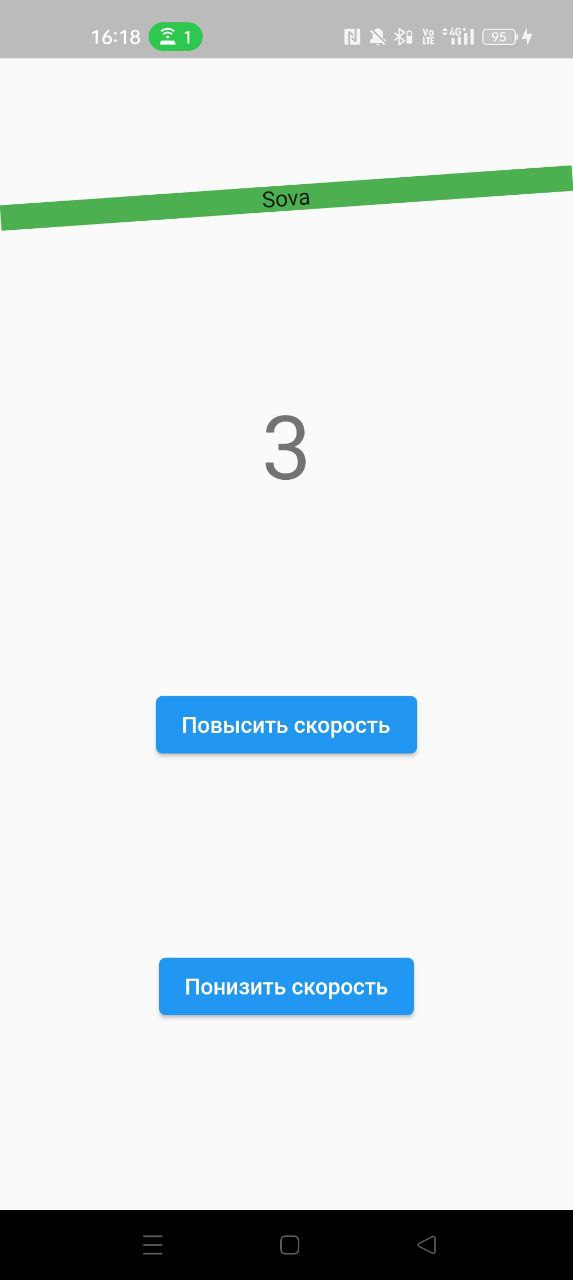
\includegraphics[width=0.5\textwidth]{images/res1.jpg}
\caption{Результат работы мобильного приложения}
\label{fig:img1}
\end{figure}


\section{Выводы}
В рамках данной лабораторной работы произошло знакомство с созданием анимации вращения на Flutter с помощью AnimationController, а также создание анимированного счетчика.
\end{document}
